\section{Schemes for computing extracellular potentials from neural activity}
\label{sec:Schemes}

The extracellular potentials that we have analyzed so far have been computed using the two-step Hodgkin-Huxley-Cable + Volume Conductor (HHC+VC) scheme (Fig. \ref{Schemes:fig:schemes}A), which is based on the theory that we presented in Chapters \ref{sec:Neuron}-\ref{sec:Sigma}. 

The HHC+VC scheme has two main limitations. Firstly, it is not self-consistent. That is, it does not compute the (intracellular) neurodynamics and the extracellular dynamics on a unified framework, and does therefore not account for so-called \textit{ephaptic effects} of extracellular variables (computed in step 2) on the neurodynamics (computed in step 1). Secondly, the HHC+VC scheme does not account for any effects that varying ion concentrations may have on the neurodynamics or on the extracellular potential, but implicitly assumes that all ion concentrations remain constant under the simulated period. 

In this chapter, we briefly summarize some alternative schemes (Fig. \ref{Schemes:fig:schemes}).
Among all existing schemes, HHC+VC is the by far most "user-friendly" scheme, and is thought to be sufficient for most purposes. However, for purposes where it is not, one should consider using one of the alternative schemes, which account ion concentration effects on the extracellular potential (Fig. \ref{Schemes:fig:schemes}B), ephaptic feedback from extracellular dynamics on neurodynamics (Fig. \ref{Schemes:fig:schemes}C) or both (Fig. \ref{Schemes:fig:schemes}D).


\begin{figure}[!ht]
\begin{center}
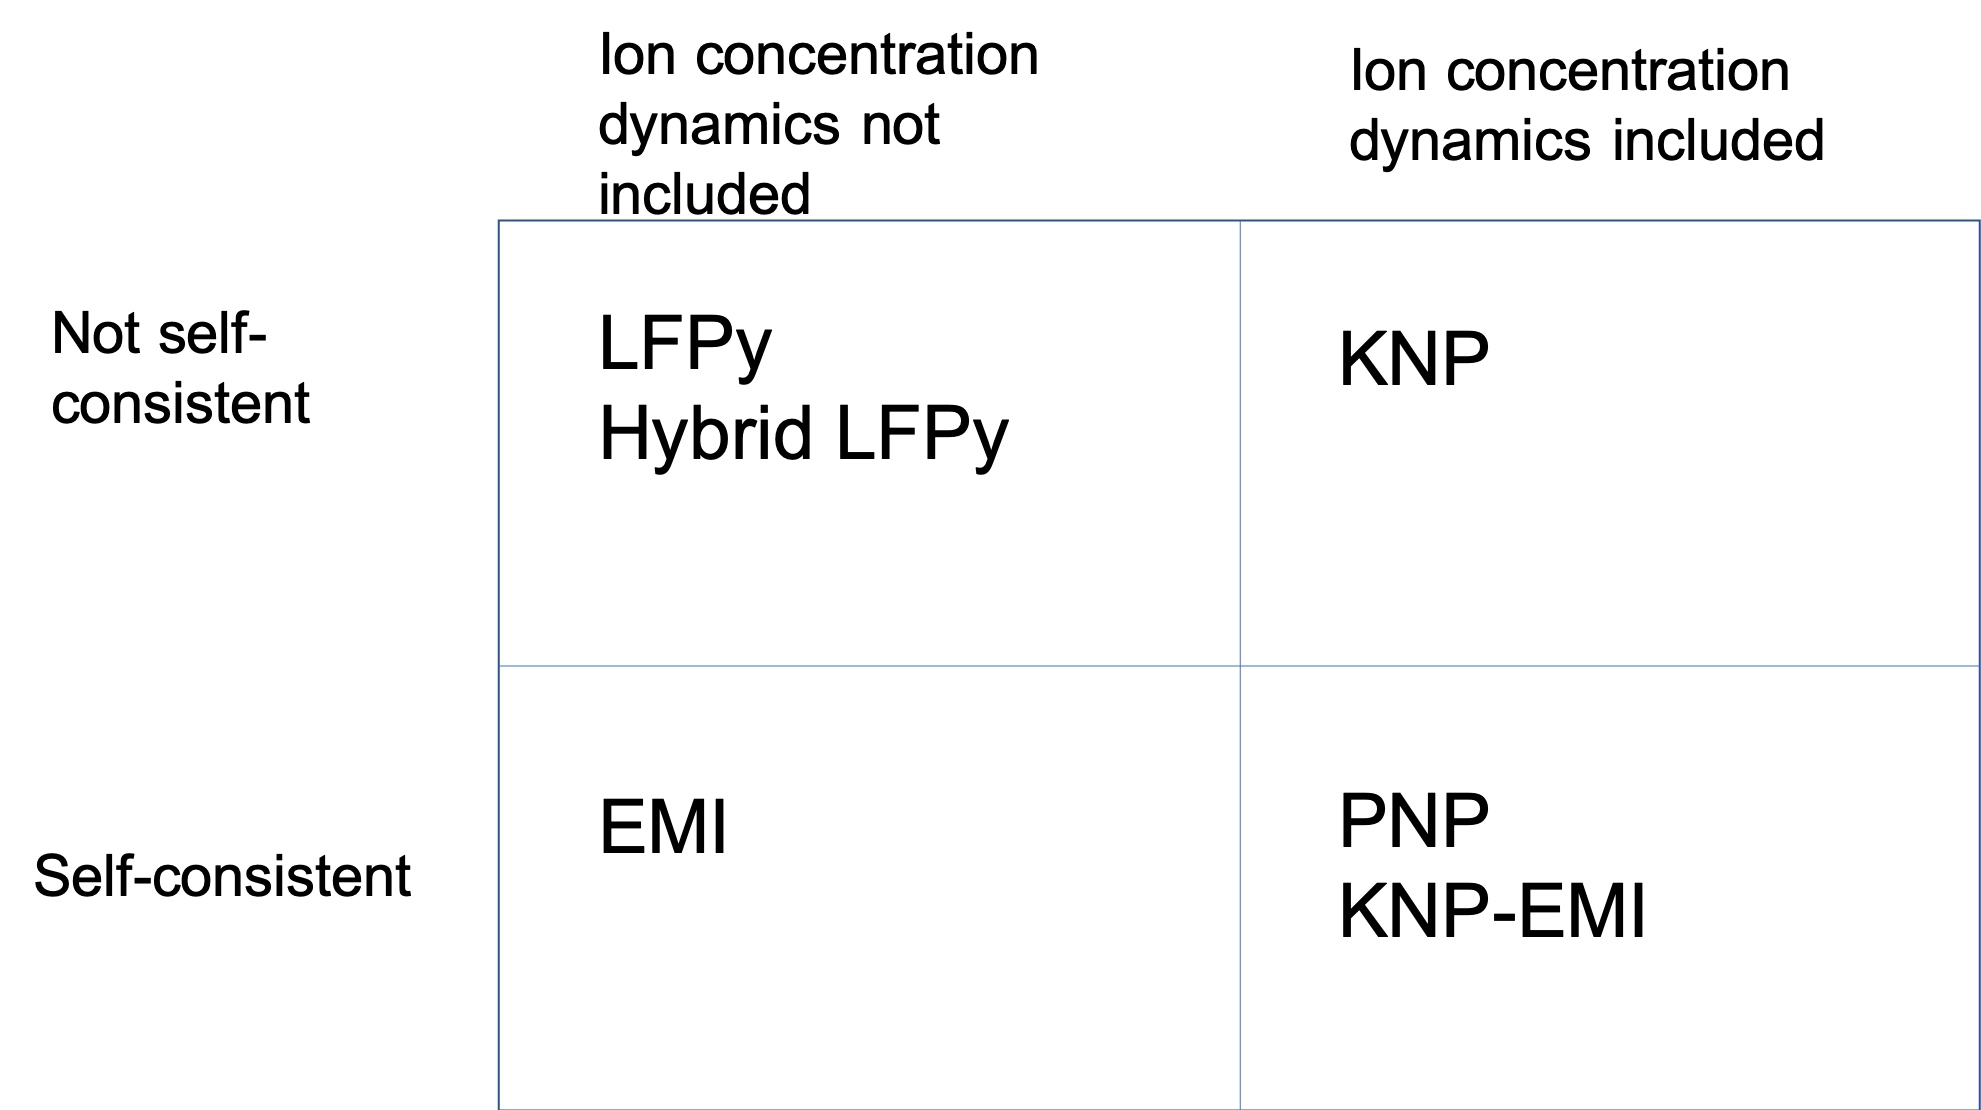
\includegraphics[width=0.8\textwidth]{Figures/Schemes/Schemes.png}
\end{center}
\caption{\textbf{Overview of schemes for computing extracellular dynamics.} The extracellular potential largely originates from neuronal transmembrane currents, illustrated for a simple (two-compartment) neuron, with currents that cross its membrane in the form of a current sink $I_1$ in one compartment, and a current source $I_2$ in the other (green arrows). {\textbf (A)}: HHC+VC: Two-step procedure which (step 1) computes transmembrane neural currents in an independent simulation using Hodgkin-Huxlley-Cable (HHC) formalism, and then (step 2) from these computes the extracellular potential using Volume Conductor (VC) theory. {\textbf (B)}: HHC + ED: Two-step scheme, which (step 1) computes currents and ion fluxes in an independent simulations based on HHC, and (step 2) from these computes the changes in the extracellular potential and ion concentrations using an electrodiffusive (ED) framework. {\textbf (C)}: VC + VC: Computes intracellular and extracellular electrodynamics simultaneously on a unified VC framework. Accounts for ephaptic effects, but assumes ion concentrations to be constant. {\textbf (D)}: ED + ED: Computes intracellular and extracellular ion concentration- and electrodynamics simultaneously on a unified electrodiffusive framework based on the Nernst-Planck equation. Account for ephaptic effects and ion-concentration dynamics. 
}
\label{Schemes:fig:schemes}
\end{figure}

When organizing the content of Part 1 of this book, we mostly followed the principle that we first present the simplest operational model, and then follow up by expanding it to more general cases and discussions of the underlying assumptions. In the current chapter, we have done things the other way around. We present the complete, self-consistent electrodiffusive schemes first (Section \ref{sec:Schemes:complete}), and follow up with the less complete schemes (Sections \ref{sec:Schemes:KNP}-\ref{sec:Schemes:VC}), showing how these can be seen as reductions of the former. 


%%%%%%%%%%%%%%%%%%


\subsection{\blue{Self-consistent electrodiffusive schemes}}
\label{sec:Schemes:complete}
\index{Electrodiffusion}
When modeling an electrodiffusive process, we keep track of the ion concentration dynamics of each individual ion species. The fundamental equation for doing that is the Nernst-Planck equation for the flux density (${\bf j_k}$ of an ion species $k$:
\begin{equation}
{\bf j_k} = - D_k {\bf \nabla} c_{k} - \frac{\tilde{D_k} z_k c_k}{\psi} {\bf \nabla} \phi, 
\label{Schemes:eq:JNP}
\end{equation}
where ${D}_k$ is the diffusion constant (units $\mathrm{m^2/s}$), $z_{k}$ is the valency of ion species $k$, and $\psi=RT/F$ (units V) is defined by the gas constant ($R$), Faraday's constant ($F$) and the temperature ($T$). The first term on the right is Fick's law for diffusion, while the second term accounts for ions migrating in the electric field. 

Ion conservation implies that:
\begin{equation}
\frac{\partial c_k}{\partial t} = -\nabla \cdot {\bf j_k},
\label{Schemes:eq:general_ionconservation}
\end{equation}
which combined with eq. \ref{Schemes:eq:JNP} gives us the Nernst-Planck continuity equation:
\begin{equation}
\frac{\partial c_k}{\partial t} = {\bf \nabla} \cdot \left[{D_k} {\bf \nabla} c_k + \frac{D_k z_k c_k}{\psi}. {\bf \nabla} \phi \right].
\label{Schemes:eq:NP}
\end{equation}

In principle, we can compute all ionic concentrations and their coupling to the electrical potential by requiring that eq. \ref{Schemes:eq:NP} should be fulfilled at all points in space, i.e., both intra- and extracellularly. Eq. \ref{Schemes:eq:NP} then gives us one equation for each individual ion concentration $c_k$, and to solve the system of equations, we are in need an additional equation for the additional variable $\phi$, the electrical potential which couples the dynamics of the individual ion species. There are two main approaches to this, the so-called \textit{Poisson-Nernst-Planck (PNP)} framework, or the so-called \textit{electroneutral} \index{Electroneutral}framework, both of which we will introduce in the following subsections. 


\subsubsection{\blue{The Poisson-Nernst-Planck (PNP) framework}}
\label{sec:Schemes:PNP}
\index{Poisson-Nernst-Planck equations}
The physically most detailed approach for defining $\phi$ in the eq. \ref{Schemes:eq:NP}) is to use Poisson's equation from electrostatics:
\begin{equation}
\nabla^2 \phi = -\rho/\epsilon
\label{Schemes:eq:poisson}
\end{equation}
Here $\epsilon$ is the permittivity of the medium, and in the last step, we have expressed the local charge density $\rho$ as a function of the ionic concentrations. 
\begin{equation}
\rho =git  F\sum_k z_k c_k.
\label{Schemes:eq:PNPrho}
\end{equation}

The PNP equations (eq. \ref{Eldiff:eq:NP} together with eq. \ref{Schemes:eq:poisson}) can in principle be solved for arbitrary complex geometries using numerical methods, like the Finite Element Method (FEM). 

To apply the PNP scheme poses several challenges. Firstly, one needs to represent the geometry and properties of the cellular membranes. In principle, this could be achieved through having spatially and temporally varying diffusion coefficients $D_k$. Membranes would then be characterized with values of $D_k$ that are (i) lower than in the extra- or intracellular bulk solution, since diffusion through membranes is constricted compared to diffusion through the bulk solutions, (ii) different in different spatial directions (i.e., normal to membrane surface versus parallel to membrane surface), and (iii) time dependent due to the opening/closing of ion channels, and varying with 

on a very fine spatial scale depending on whether or not there are ion channels present at a particular patch of membrane. 

Unless the PNP scheme is applied to specifically model currents inside ion channels on a very small spatial scale (see e.g., \citep{Gardner2011, Zheng2011}), such a fine-grained tensor description of $D_k$ will 

it is common to rather have the PNP equations being defined in two disjoint domains - the intra and extracellular - and to couple the dynamics in these two domains by introducing suitable boundary conditions at the membrane manifold. In many applications, the membrane dynamics is then instead described using a Hodgkin-Huxley (HH) type formalism (c.f., Section \ref{sec:Neuron:membranecurrents}) also in PNP type modeling (see e.g., \citep{Lopreore2008, Pods2013, Gardner2015, Pods2017}). When applying a HH formalism in this context, all transmembrane currents must be made ion specific, i.e., they must be described in terms of ionic fluxes over the membrane, so that for example a Na$^+$ current density ($i_{Na}$) in the standard HH formalism would need to be replaced with a Na$^+$ flux density, $j_{Na} = i_{Na}/(Fz_k)$. Apart from that, the HH formalism for membrane mechanisms can be applied in its original form also in an electrodiffusive context.

Secondly, solving the PNP system of equations is extremely computationally demanding. One reason for this is that the concentrations of ions in a finite volume of space are almost so that the net positive and negative charges outbalance, meaning that the medium is very close to electroneutral. A non-zero charge density ($\rho$) thus reflects a deviance from electronutrality, and it has been estimated that this deviance typically involves only a fraction $\sim 10^{-9}$ of the ions present \citep{Aguilella1987}. An accurate prediction of $\rho$ from eq. \ref{Schemes:eq:PNPrho} thus requires an extreme precision in the modeling of the ionic concentrations $c_k$. Another reason, as we discussed briefly in Section \ref{sec:Eldiff:LJpot}, is that the charge-relaxation time in the extracellular solution, i.e., the time scale that $\rho$ varies on, is in the order of nanoseconds. In addition, any non-zero charge density in neural tissue is predominantly resolved in nano-meter thick layers around neuronal membranes \citep{Grodzinsky2011, Gratiy2017}. Simulations of $\rho$ therefore require a spatiotemporal resolution smaller than nanometers and nanoseconds, and thus a very fine-grained description of the tissue where neuronal, glial and extracellular geometries are explicitly defined.

Due to its computational demand, the PNP framework is not suitable for estimating dynamics at the level of tissue, and the framework does not lend itself to be coarse-grained. Applications in neuroscience have therefore been limited to studies of electrodiffusive processes taking place on a very tiny spatiotemporal scale near and inside membranes (see e.g., \citep{Leonetti2004, Lu2007, Lopreore2008, Nanninga2008, Gardner2011, Zheng2011, Pods2013, Gardner2015}). See \citep{Savtchenko2017} for a review of applications in neuroscience.


\subsubsection{\blue{The electroneutral framework}}
\label{sec:Schemes:electroneutral}
\index{Electroneutral}
An alternative to the PNP framework is to replace the Poisson equation (eq. \ref{Eldiff:eq:poisson}) with the approximation that the bulk solution is electroneutral:
\begin{equation}
F \sum_k z_k c_k = 0.
\label{Schemes:eq:electroneutral}
\end{equation}
In practice, it is often more convenient to impose the electroneutrality approximation on differential form:
\begin{equation}
F \sum_k{z_k \frac{\partial c_k}{\partial t}} = 0.
\label{Schemes:eq:electroneutral2}
\end{equation}

The electroneutrality approximation (eq. \ref{Schemes:eq:electroneutral} or \ref{Schemes:eq:electroneutral2}) can be imposed as a constraint when solving eq.\ref{Schemes:eq:NP} by use of some numerical method. The constraint is then used to determine the value that $\phi$ must have for there to be no charge accumulation anywhere in the extracellular or intracellular bulk solutions, a problem which has a unique solution. 

To explain how this differs from the PNP framework, we may use our previous cartoon example (Fig. \ref{Eldiff:fig:diffpot}) as a reference. While the PNP framework explicitly models the nanosecond-fast charge relaxation process (Fig. \ref{Eldiff:fig:diffpot}B), the electroneutral scheme circumvents this by assuming (and ensuring) that the system is always in quasi-steady (Fig. \ref{Eldiff:fig:diffpot}C). It has been shown that this is a good approximation on spatiotemporal scales larger than micrometers and microseconds \citep{Grodzinsky2011, Pods2017, Solbra2018}. The advantage with this approach is that it, unlike PNP, gives stable solutions with an arbitrary coarse spatiotemporal resolution.

We note that the electroneutrality constraint (eq. \ref{Schemes:eq:electroneutral} or \ref{Schemes:eq:electroneutral2}) only applies to the intra- and extracellular bulk solutions, so that the membrane dynamics must be dealt with separately. Firstly, one must define the equations that govern the membrane dynamics. A natural choice for this is, again, to use an ion-specific HH-like formalism \citep{Mori2006, Mori2009, Pods2017, ellingsrud2020}. 

Secondly, the electroneutrality condition does not apply at the membrane, where a non-zero charge density ($\rho_{m}$) builds up the membrane potential according to the capacitor relationship:
\begin{equation}
C_m \phi_{m} = \pm \rho_{mr},
\label{Schemes:eq:rhocap}
\end{equation}
where $r$ takes the indexes $i$ (intracellular side of the membrane) or $e$ (extracellular side of the membrane), and where the plus-sign should be used for $r=i$, and the minus-sign for $r=e$, a convention that follows from the definition $\phi_{m} = \phi_{i} - \phi_{e}$. The intra- and extracellular membrane charge densities in eq. \ref{Schemes:eq:rhocap} are equal in magnitude and opposite in sign, since the charge stored on one side of a capacitor always balances the charge stored on the other side. 

A technical challenge when implementing the electroneutral framework is that, while eq. \ref{Schemes:eq:rhocap} uniquely determines what  $\rho^{mr}$ must be for a given $\phi_{m}$, it does not uniquely determine the composition of ions that gives rise to this  $\rho^{mr}$. When implementing the electroneutral framework, one must keep track of all ionic movements, and therefore also make some assumption as to which ions that actually constitute the membrane charge. In previous implementations, two different approaches has been taken to this:

\begin{itemize}

\item In the approach (A1) taken by Mori and Peskin \citep{Mori2006, Mori2009}, also used by Pods \citep{Pods2017}, a set of additional state variables ($c_k^{mr}$) were defined for the membrane ion concentrations. These were defined so that they (i) summed up to the correct membrane charge density: 
\begin{equation}
\rho_{m}^r = F \sum_k z_k c_k^{mr},
\label{Schemes:eq:rhomem}
\end{equation}
and (ii) so that the ratio between the membrane concentrations $c_k^{mr}$ of the various ion species $k$ was roughly the same as the ratio between the various species $c_k^r$ in the bulk solution close to the membrane on either side. 

\item In the approach (A2) by Ellingsrud et al. \citep{ellingsrud2020}, which they there referred to as the Kirchhoff-Nernst-Planck + Extracellular-Membrane-Intracellular (KNP-EMI) scheme, the membrane boundary condition was instead based on (i) using the differential form of eq. \ref{Schemes:eq:rhocap}:
\begin{equation}
I_{cap}^r = \pm \frac{\partial \rho_{m}^r}{\partial dt}, 
\label{Schemes:eq:rhocap2}
\end{equation}
where the left hand side followed from the definition of the capacitive membrane current (cf. eq. \ref{Neuron:eq:HHcap}). $I_{cap}$, which is given by the membrane potential dynamics computed with the a HH-type framework, was then (ii) made ion specific, and defined so that the ratio between the contributions ($I^k_{cap}$) from the various ion species $k$ was identical to the ratio between the various species $c_k^r$ in the bulk solution close to the membrane at either side.
\end{itemize}

Although they differ in implementation details, the two approaches (A1 and A2) should be close to equivalent from a physics point of view. In practice, only a very tiny fraction of the ions present are involved in building up the membrane potential, and the choice as to which ion species that actually constitute the membrane charge in eq. \ref{Schemes:eq:rhomem} or \ref{Schemes:eq:rhocap2} is probably quite unimportant for the overall system dynamics. The choice should rather be regarded as a technicality, made to ensure ion conservation and a consistent charge-concentration relationship at all points in space. 

Like the PNP scheme, both versions of the electroneutral scheme must be solved on some numerical framework using a suitable meshing of the tissue volume. While the electroneutral frameworks are computationally much more efficient than the PNP framework, they are still too heavy to allow for simulations of large systems of neurons described with explicit geometries on today's computers. To our knowledge, the largest system that so far has been simulated in 3D on an electroneutral framework is small piece of tissue containing a bundle of 9 axons described with idealized geometries \citep{ellingsrud2020}.



\subsubsection{\blue{Domain models}}
\label{sec:Schemes:domain}
\index{Domain models}
A different category of electroneutral models have been inspired from by the bi-domain model by Eisenberg \citep{eisenberg1970}, which has previously been used to simulate cardiac tissue \citep{henriquez1993, sundnes2006, Mori2008}. 

In this category, the most advanced models for brain tissue are the tri-domain models, where three the domains represent (i) neurons, (ii) extracellular space, and (iii) a glial syncytium, i.e., a populations of gap-junction coupled glial cells \citep{OConnell2016, tuttle2019}. In the domain models, geometry is not explicitly accounted for. Instead, all domains "exist" at each point in space, and are defined through a set of domain-specific variables (e.g., domain-voltage, domain-ion concentrations, domain-volume fractions). The domains interact locally through a set of (Hodgkin-Huxley type) membrane mechanisms, while spatial electrodiffusive transports occurs within the domains. By assumption, ion transport through the glial syncytium equivalent to extracellular transport, i.e., it can occur in a spatially continuous fashion through a (tortous) intracellular space involving many interconnected cells. In contrast, neurons are "local" in the sense that no intracellular transport over distances occur within the neural domain (Fig.\ref{Schemes:fig:domainmodel}). 

\begin{figure}[!ht]
\begin{center}
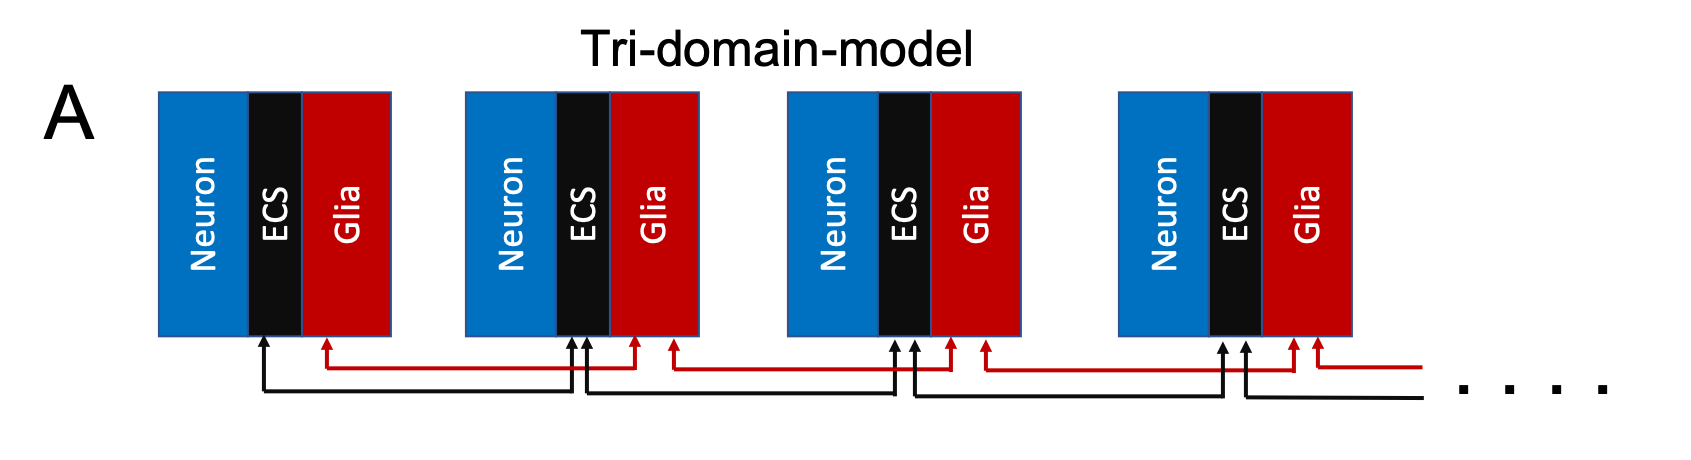
\includegraphics[width=0.8\textwidth]{Figures/Schemes/Tridomain.png}
\end{center}
\caption{\textbf{Tri-domain model of brain tissue.} The domains represent neurons, extracellular space (ECS) and glial cells. The domains interact locally through transmembrane currents. Spatial ellectrodiffusion (arrows) occur within the ECS and glia domains, but not in within neuronal domain.The spatial dynamics can, in principle, occur in all directions (3D),but a 1D illustration was used in the figure. 
}
\label{Schemes:fig:domainmodel}
\end{figure}

Simpler, related models include the bi-domain model for neurons and extracellular space \citep{Mori2015}, or 1D models of glial K$^+$ buffering, where only the glial and extracellular domain were included \cite{Gardner-Medwin1983, Chen2000, Halnes2013}.

Domain models are suited to model brain dynamics taking place on a slow time-scale, such as the wave of K$^+$ and the slow, DC-like diffusion potentials and glial buffering potentials that take place during speading depression \citep{Mori2015, OConnell2016, tuttle2019}. As these models treat brain tissue as a homogeneous, coarse-grained continuum, they are not suited to model the faster fluctuations of extracellular potentials which are recorded in MUA, LFP and EEG, as these depend strongly on morphologies of neurons \citep{Einevoll2013}. 





%%%%%%%%%%%%%%%%%%%%%%%%%%%%%%%%%%%%%%%%%%%%%

%%%%%%%%%%%%%%%%%%%%%%%%%%%%%%%%%%%%%%%%%%%


\subsection{\blue{Self-consistent volume conduction scheme}}
The self-consistent (VC+VC) scheme models both intra- and extracellular electrodynamics by Ohmic volume conduction:
\begin{equation}
\nabla \cdot \sigma_r \nabla \phi_r
\end{equation}
where $r$ takes the indexes $i$ (intracellular space) or $e$ (extracellular space). The intra- and extracellular dynamics are coupled through suitable boundary mechanisms at the membrane, i.e., a current \textit{entering} the membrane (normal component) at one side of the membrane, is constrained to be identical to the current \textit{leaving} the membrane (negative normal component) on the opposite side  \citep{Krassowska1994}. These entering and leaving currents are in turn determined by the transmembrane current $I_m$, which, again, in most applications are modeled with Hodgkin-Huxley like kinetics \citep{Agudelo-Toro2013, Tveito2017}. 

Unlike the standard two-step HHC+VC framework, the VC+VC framework accounts for the ephaptic effect \index{Ephaptic effects} from the extracellular potential on the neuronal membrane potential dynamics. As such, VC+VC is the more complete framework. However, it has the disadvantage that it is computationally expensive. In the HHC + VC scheme, which uses volume conduction modeling only for the extracellular space, $\phi_e$ can be computed as an analytical function of the transmembrane neural currents (cf. Chapter \ref{sec:VC}). Analytical examples of solutions have also been obtained with the VC+VC scheme for idealized scenarios 
 \citep{Krassowska1994}, but general applications of VC+VC require that both the intra- and extracellular spaces are spatially resolved and their dynamics computed on a numerical framework \citep{Agudelo-Toro2013, Tveito2017}. 

Using VC+VC to simulate larger systems with realistic morphologies would probably exceed the capacity of today's computers. However, VC+VC has been used to perform a systematic exploration of the inaccuracies induced when ignoring ephaptic effects in a small system of neurons represented with stylized geometries  \citep{Tveito2019}.


%%%%%%%%%%%%%%%%%%%%%%%%%%%%%%%%%%%%%%%%%%%


\subsection{\blue{Two-step scheme: Hodgkin-Huxley-Cable + Electrodiffusion}}
\label{sec:Schemes:KNP}
By necessity, the transmembrane ionic currents that mediate neurodynamics will lead to changes in the intra- and extracellular ion concentrations. Under normal circumstances, these changes are limited to small deviances from baseline, since neurons and glial cells contain numerous homeostatic mechanisms that work continuously to restore baseline concentrations. However, during neuronal hyperactivity, or during several pathological conditions, the homeostatic machinery can fail to keep up, and ion concentrations may then change rather dramatically, both in the intra- and extracellular space \citep{Dietzel1989, Somjen2001, Frohlich2008, Zandt2015, Ayata2015}. This will in turn change the neuronal reversal potentials (cf. eq. \ref{Neuron:eq:revpots}), and through that alter the neuronal firing properties, something that has been the topic of several studies (see e.g., \citep{Qian1989, Cressman2009, Zandt2011, Oyehaug2012, WeiUllahSchiff2014, Saetra2020}). Local changes in extracellular concentrations will also give rise to diffusive currents along extracellular concentration gradients. These will in turn generate diffusion potentials. Under such circumstances, the extracellular potential ($\phi_e$) is not solely a function of cellular transmembrane currents (as assumed when using VC theory), but also contains contribution from extracellular diffusion \citep{Halnes2016}. 

The HHC+ED scheme is a two-step scheme developed to compute the dynamics in the extracellular space, when when "receiving" input from discrete neuronal sources. Like the standard HHC+VC-scheme, the HHC+ED does not account for any feedback effects from the $\phi_e$ or ion concentrations on the neurodynamics. However, unlike the standard HHC+VC scheme, it computes the dynamics of extracellular ion concentrations and accounts for their effects on $\phi_e$. In the one existing implementation of this scheme, the extracellular dynamics was computed using the so-called electroneutral \index{Electroneutral} electrodiffusive \index{Electrodiffusion} Kirchhoff-Nernst-Planck (KNP) framework \citep{Solbra2018}. 

\begin{figure}[!ht]
\begin{center}
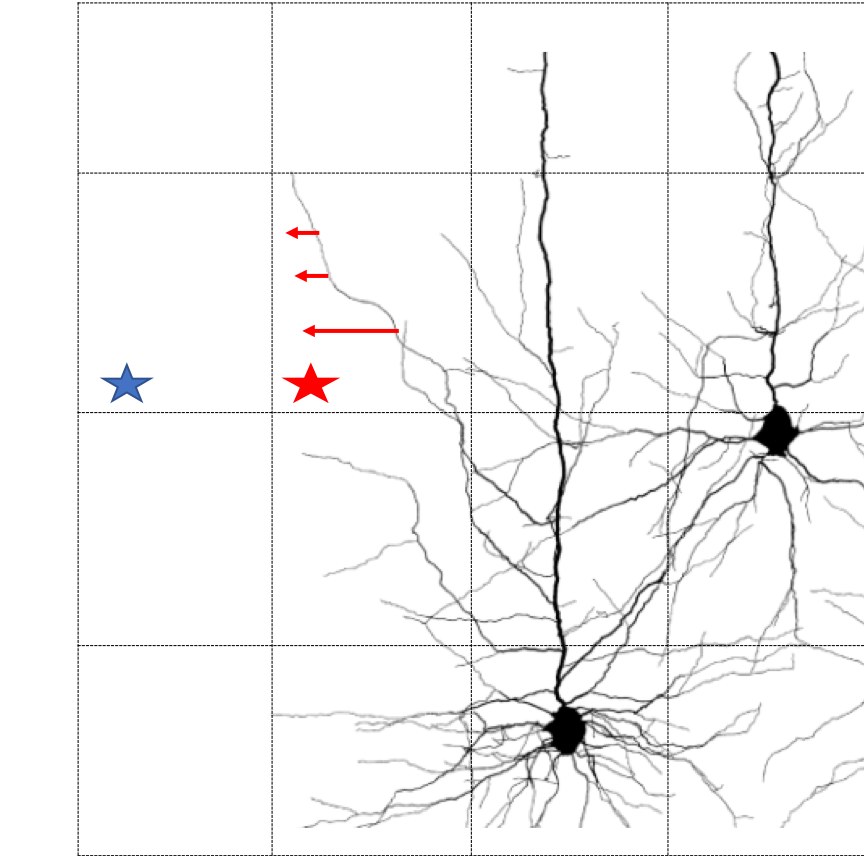
\includegraphics[width=0.5\textwidth]{Figures/Eldiff/KNP.png}
\end{center}
\caption{\textbf{KNP scheme}. Blue star: Mesh cell containing no neuronal sources, so that $C=0$. Red star: Mesh cell containing neural sources. Here $C$ can be computed by summing over all neuronal transmembrane currents, including the capacitive current, and dividing by the volume of the mesh cell. \ghnote{LAGE LITT MER INFORMATIV FIG HER OM VI SKAL HA FIG HER.}}
\label{Eldiff:fig:KNPmesh}
\end{figure}

The HHC+ED can be summarized as follows:

\begin{itemize}
\item {\bf Step 1:} Compute neurodynamics using a standard HHC-type framework (Chapter \ref{sec:Neuron}). Unlike in the standard HHC+VC scheme, where the different kinds of transmembrane currents, such as leakage currents, capacitive currents, and ion specific active currents, can be grouped into a single source variable $C$ for the total CSD at each segment, the HHC+ED scheme requires that all neural sources are expressed as a set of ion specific fluxes, i.e., one source $f_k$ per ion species $k$ and an additional capacitive neuronal membrane current source density, $C_{cap}$, the only source term not accounted for in the set $f_k$.

\item {\bf Step 2:} Use the electrodiffusive KNP framework to compute the voltage and ion concentration dynamics in the extracellular space, when "receiving" input from discrete neuronal sources computed in Step 1.
\end{itemize}

The KNP scheme used in (Step 2) is a method for solving the extracellular ion concentration dynamics that we introduced in Chapter \ref{sec:Eldiff}, and the fundamental equation: 
\begin{equation}
\alpha \frac{\partial c_k}{\partial t} = {\bf \nabla} \cdot \left[ \tilde{D_k} {\bf \nabla} c_k + \frac{\tilde{D_k} z_k c_k}{\psi} {\bf \nabla} \phi \right] + f_k,
\label{Schemes:eq:NPe}
\end{equation}
is the Nernst-Planck equation in on the same form that we used earlier (eq. \ref{Eldiff:eq:NPe}). We recall that $\alpha$ is the extracellular volume fraction, and $\tilde{D_k}$ is the effective diffusion constant for ions in the (coarse-grained) extracellular space. As all variables are extracellular, we have skipped the indexing. 

To solve this set of equations (one instance of eq. \ref{Eldiff:eq:NPe} for each ion species $k$), we need an additional constraint for the additional variable $\phi$. To account for capacitive sources, i.e., charge accumulation at neural membranes, we use the constraint:
\begin{equation}
\alpha F \sum_k{z_k \frac{\partial c_k}{\partial t}} = C_{cap},
\label{Schemes:eq:electroneutral3}
\end{equation}
where the (neural) capacitive current source density:
\begin{equation}
C_{cap} = {\alpha}\frac{\partial \rho_{mem}}{\partial dt},
\label{Schemes:eq:Andreas}
\end{equation}
reflects the membrane potential dynamics of a neuron due to charge accumulating on the membrane surface. As $C_{cap}$ is zero at all locations where there is no neuronal membrane source, the bulk solution of the extracellular space will be electroneutral, i.e., the ionic concentrations will sum up to a zero charge density:
\begin{equation}
\sum_k{z_k \frac{\partial c_k}{\partial t}} = 0.
\label{Schemes:eq:electroneutral4}
\end{equation}
We will comment further on the electroneutrality condition in Section \ref{sec:Schemes:complete}.

The constraint in eq. \ref{Schemes:eq:electroneutral3} was essentially what we used in Chapter \ref{sec:Eldiff} to get from eq. \ref{Eldiff:eq:chargecontinuity} to eq. \ref{Eldiff:eq:eldiffCSD2}. The KNP scheme thus uses Eq. \ref{Eldiff:eq:eldiffCSD2} with $C$ as defined in eq.  \ref{Eldiff:eq:CSDdecomposed} to to derive $\phi$:
\begin{equation}
\nabla \cdot (\sigma\nabla\phi) = - F \sum_k z_k f_k -  C_{cap} - F\alpha \nabla \cdot \left (\sum_k{z_k \tilde{D_k}{\bf \nabla} c_{k}} \right).
\label{Schemes:eq:KNPfinal}
\end{equation}
Through this equation, $\phi$ is uniquely determined by the ion concentrations ($c_k$) and the neuronal CSD, and with that, the Nernst-Planck equations (eq. \ref{Schemes:eq:NPe}) can be solved on a suitable numerical framework.


%%%%%%%%%%%%%%%%%%%%%%%%%%%%%%%%%%%%%%%%


